\documentclass{article}
\usepackage{amsmath}
\usepackage{changepage}
\usepackage{float}
\usepackage{amsmath}
\usepackage{tikz}
\usepackage{graphicx}
\usepackage{color}
\usepackage{listings}
\usepackage{color}
\usepackage{algpseudocode}
\definecolor{dkgreen}{rgb}{0,0.6,0}
\definecolor{gray}{rgb}{0.5,0.5,0.5}
\definecolor{mauve}{rgb}{0.58,0,0.82}
\usetikzlibrary{arrows}

\lstset{frame=tb,
  language=Java,
  aboveskip=3mm,
  belowskip=3mm,
  showstringspaces=false,
  columns=flexible,
  basicstyle={\small\ttfamily},
  numbers=none,
  numberstyle=\tiny\color{gray},
  keywordstyle=\color{blue},
  commentstyle=\color{dkgreen},
  stringstyle=\color{mauve},
  breaklines=true,
  breakatwhitespace=true,
  tabsize=3
}

\long\def\/*#1*/{}

\tikzset{
  treenode/.style = {align=center, inner sep=0pt, text centered,
    font=\sffamily},
  1/.style = {treenode, circle, white, font=\sffamily\bfseries, draw=black,
    fill=black, text width=1.5em},% arbre rouge noir, noeud noir
  2/.style = {treenode, circle, white, draw=black, 
    text width=1.5em, very thick},% arbre rouge noir, noeud rouge
  3/.style = {treenode, circle, white, draw=black,
    minimum width=0.5em, minimum height=0.5em}% arbre rouge noir, nil
}
\tikzset{
  treenode/.style = {align=center, inner sep=0pt, text centered,
    font=\sffamily},
  arn_n/.style = {treenode, circle, white, font=\sffamily\bfseries, draw=black,
    fill=black, text width=1.5em},% arbre rouge noir, noeud noir
  arn_r/.style = {treenode, circle, red, draw=red, 
    text width=1.5em, very thick},% arbre rouge noir, noeud rouge
  arn_x/.style = {treenode, rectangle, draw=black,
    minimum width=0.5em, minimum height=0.5em}% arbre rouge noir, nil
}
\begin{document}
\begin{center}
Andreas Bach Landgrebe \\
Computer Science 250: Analysis of Algorithms \\
March 3, 2015 \\
Laboratory Assignment 6 -   – Trees  \\
\end{center}
\newpage
\noindent
\begin{center}
\textbf{Part One: Traversing Binary Search Trees \\ Source Code}
\end{center}
\begin{lstlisting}
/*************************************************************************
 *  Compilation:  javac BST.java
 *  Execution:    java BST
 *  Dependencies: StdIn.java StdOut.java Queue.java
 *  Data files:   http://algs4.cs.princeton.edu/32bst/tinyST.txt
 *
 *  A symbol table implemented with a binary search tree.
 *
 *  % more tinyST.txt
 *  S E A R C H E X A M P L E
 *
 *  % java BST < tinyST.txt
 *  A 8
 *  C 4
 *  E 12
 *  H 5
 *  L 11
 *  M 9
 *  P 10
 *  R 3
 *  S 0
 *  X 7
 *
 *************************************************************************/

import java.util.NoSuchElementException;
import java.util.*;
import java.io.*; //added some import statement just in case

public class BST<Key extends Comparable<Key>, Value> {
    private Node root;             // root of BST

    private class Node {
        private Key key;           // sorted by key
        private Value val;         // associated data
        private Node left, right;  // left and right subtrees
        private int N;             // number of nodes in subtree

        public Node(Key key, Value val, int N) {
            this.key = key;
            this.val = val;
            this.N = N;
        }
    }

    // is the symbol table empty?
    public boolean isEmpty() {
        return size() == 0;
    }

    // return number of key-value pairs in BST
    public int size() {
        return size(root);
    }

    // return number of key-value pairs in BST rooted at x
    private int size(Node x) {
        if (x == null) return 0;
        else return x.N;
    }

   /***********************************************************************
    *  Search BST for given key, and return associated value if found,
    *  return null if not found
    ***********************************************************************/
    // does there exist a key-value pair with given key?
    public boolean contains(Key key) {
        return get(key) != null;
    }

    // return value associated with the given key, or null if no such key exists
    public Value get(Key key) {
        return get(root, key);
    }

    private Value get(Node x, Key key) {
        if (x == null) return null;
        int cmp = key.compareTo(x.key);
        if      (cmp < 0) return get(x.left, key);
        else if (cmp > 0) return get(x.right, key);
        else              return x.val;
    }

   /***********************************************************************
    *  Insert key-value pair into BST
    *  If key already exists, update with new value
    ***********************************************************************/
    public void put(Key key, Value val) {
        if (val == null) { delete(key); return; }
        root = put(root, key, val);
        assert check();
    }

    private Node put(Node x, Key key, Value val) {
        if (x == null) return new Node(key, val, 1);
        int cmp = key.compareTo(x.key);
        if      (cmp < 0) x.left  = put(x.left,  key, val);
        else if (cmp > 0) x.right = put(x.right, key, val);
        else              x.val   = val;
        x.N = 1 + size(x.left) + size(x.right);
        return x;
    }

   /***********************************************************************
    *  Delete
    ***********************************************************************/

    public void deleteMin() {
        if (isEmpty()) throw new NoSuchElementException("Symbol table underflow");
        root = deleteMin(root);
        assert check();
    }

    private Node deleteMin(Node x) {
        if (x.left == null) return x.right;
        x.left = deleteMin(x.left);
        x.N = size(x.left) + size(x.right) + 1;
        return x;
    }

    public void deleteMax() {
        if (isEmpty()) throw new NoSuchElementException("Symbol table underflow");
        root = deleteMax(root);
        assert check();
    }

    private Node deleteMax(Node x) {
        if (x.right == null) return x.left;
        x.right = deleteMax(x.right);
        x.N = size(x.left) + size(x.right) + 1;
        return x;
    }

    public void delete(Key key) {
        root = delete(root, key);
        assert check();
    }

    private Node delete(Node x, Key key) {
        if (x == null) return null;
        int cmp = key.compareTo(x.key);
        if      (cmp < 0) x.left  = delete(x.left,  key);
        else if (cmp > 0) x.right = delete(x.right, key);
        else {
            if (x.right == null) return x.left;
            if (x.left  == null) return x.right;
            Node t = x;
            x = min(t.right);
            x.right = deleteMin(t.right);
            x.left = t.left;
        }
        x.N = size(x.left) + size(x.right) + 1;
        return x;
    }


   /***********************************************************************
    *  Min, max, floor, and ceiling
    ***********************************************************************/
    public Key min() {
        if (isEmpty()) return null;
        return min(root).key;
    }

    private Node min(Node x) {
        if (x.left == null) return x;
        else                return min(x.left);
    }

    public Key max() {
        if (isEmpty()) return null;
        return max(root).key;
    }

    private Node max(Node x) {
        if (x.right == null) return x;
        else                 return max(x.right);
    }

    public Key floor(Key key) {
        Node x = floor(root, key);
        if (x == null) return null;
        else return x.key;
    }

    private Node floor(Node x, Key key) {
        if (x == null) return null;
        int cmp = key.compareTo(x.key);
        if (cmp == 0) return x;
        if (cmp <  0) return floor(x.left, key);
        Node t = floor(x.right, key);
        if (t != null) return t;
        else return x;
    }

    public Key ceiling(Key key) {
        Node x = ceiling(root, key);
        if (x == null) return null;
        else return x.key;
    }

    private Node ceiling(Node x, Key key) {
        if (x == null) return null;
        int cmp = key.compareTo(x.key);
        if (cmp == 0) return x;
        if (cmp < 0) {
            Node t = ceiling(x.left, key);
            if (t != null) return t;
            else return x;
        }
        return ceiling(x.right, key);
    }

   /***********************************************************************
    *  Rank and selection
    ***********************************************************************/
    public Key select(int k) {
        if (k < 0 || k >= size()) return null;
        Node x = select(root, k);
        return x.key;
    }

    // Return key of rank k.
    private Node select(Node x, int k) {
        if (x == null) return null;
        int t = size(x.left);
        if      (t > k) return select(x.left,  k);
        else if (t < k) return select(x.right, k-t-1);
        else            return x;
    }

    public int rank(Key key) {
        return rank(key, root);
    }

    // Number of keys in the subtree less than key.
    private int rank(Key key, Node x) {
        if (x == null) return 0;
        int cmp = key.compareTo(x.key);
        if      (cmp < 0) return rank(key, x.left);
        else if (cmp > 0) return 1 + size(x.left) + rank(key, x.right);
        else              return size(x.left);
    }

   /***********************************************************************
    *  Range count and range search.
    ***********************************************************************/
    public Iterable<Key> keys() {
        return keys(min(), max());
    }

    public Iterable<Key> keys(Key lo, Key hi) {
        Queue<Key> queue = new Queue<Key>();
        keys(root, queue, lo, hi);
        return queue;
    }

    private void keys(Node x, Queue<Key> queue, Key lo, Key hi) {
        if (x == null) return;
        int cmplo = lo.compareTo(x.key);
        int cmphi = hi.compareTo(x.key);
        if (cmplo < 0) keys(x.left, queue, lo, hi);
        if (cmplo <= 0 && cmphi >= 0) queue.enqueue(x.key);
        if (cmphi > 0) keys(x.right, queue, lo, hi);
    }

    public int size(Key lo, Key hi) {
        if (lo.compareTo(hi) > 0) return 0;
        if (contains(hi)) return rank(hi) - rank(lo) + 1;
        else              return rank(hi) - rank(lo);
    }


    // height of this BST (one-node tree has height 0)
    public int height() { return height(root); }
    private int height(Node x) {
        if (x == null) return -1;
        return 1 + Math.max(height(x.left), height(x.right));
    }


    // level order traversal
    public Iterable<Key> levelOrder() {
        Queue<Key> keys = new Queue<Key>();
        Queue<Node> queue = new Queue<Node>();
        queue.enqueue(root);
        while (!queue.isEmpty()) {
            Node x = queue.dequeue();
            if (x == null) continue;
            keys.enqueue(x.key);
            queue.enqueue(x.left);
            queue.enqueue(x.right);
        }
        return keys;
    }

  /*************************************************************************
    *  Check integrity of BST data structure
    *************************************************************************/
    private boolean check() {
        if (!isBST())            StdOut.println("Not in symmetric order");
        if (!isSizeConsistent()) StdOut.println("Subtree counts not consistent");
        if (!isRankConsistent()) StdOut.println("Ranks not consistent");
        return isBST() && isSizeConsistent() && isRankConsistent();
    }

    // does this binary tree satisfy symmetric order?
    // Note: this test also ensures that data structure is a binary tree since order is strict
    private boolean isBST() {
        return isBST(root, null, null);
    }

    // is the tree rooted at x a BST with all keys strictly between min and max
    // (if min or max is null, treat as empty constraint)
    // Credit: Bob Dondero's elegant solution
    private boolean isBST(Node x, Key min, Key max) {
        if (x == null) return true;
        if (min != null && x.key.compareTo(min) <= 0) return false;
        if (max != null && x.key.compareTo(max) >= 0) return false;
        return isBST(x.left, min, x.key) && isBST(x.right, x.key, max);
    }

    // are the size fields correct?
    private boolean isSizeConsistent() { return isSizeConsistent(root); }
    private boolean isSizeConsistent(Node x) {
        if (x == null) return true;
        if (x.N != size(x.left) + size(x.right) + 1) return false;
        return isSizeConsistent(x.left) && isSizeConsistent(x.right);
    }

    // check that ranks are consistent
    private boolean isRankConsistent() {
        for (int i = 0; i < size(); i++)
            if (i != rank(select(i))) return false;
        for (Key key : keys())
            if (key.compareTo(select(rank(key))) != 0) return false;
        return true;
    }


    /****************************************************************************
    * In Order Traversal Methods
    *****************************************************************************/

    public void InOrderTraversal(){
    	InOrderTraversal(root);

    }//InOrderTraversal Method

    public void InOrderTraversal (Node j) {
    	if (j == null){
    		return;
    	}//if

    	InOrderTraversal(j.left);

    	System.out.println("(" + j.key + " , " + j.val + ")");

    	InOrderTraversal(j.right);

    } // InOrderTraversal Method

    /****************************************************************************
    * Pre Order Traversal Methods
    *****************************************************************************/

    public void PreOrderTraversal() {

    	PreOrderTraversal(root);

    } //PreOrderTraversal method

    public void PreOrderTraversal(Node k){

    	if (k == null){
    		return;
    	} //if 

    	System.out.println("(" + k.key + "," + k.val + ")");

    	PreOrderTraversal(k.left);
    	PreOrderTraversal(k.right);
    } //PreOrderTraversal method


    /****************************************************************************
    * Post Order Traversal Methods
    *****************************************************************************/

    public void PostOrderTraversal() {

    	PostOrderTraversal(root);

    }//PostOrderTraversal method	

    public void PostOrderTraversal(Node l){
    	if (l == null){
    		return;
    	} // if

    	PostOrderTraversal(l.left);
    	PostOrderTraversal(l.right);

    	System.out.println("(" + l.key + "," + l.val + ")");

    }

   /*****************************************************************************
    *  Test client
    *****************************************************************************/
   public static void main(String[] args) {
   	BST<String, Integer> st = new BST<String, Integer>();
   	for (int i = 0; !StdIn.isEmpty(); i++) {
   		String key = StdIn.readString();
   		st.put(key, i);
   	}

        //Scanner scan = new Scanner(System.in);

        //System.out.println("What Kind of Travesal Method Would You Like To Do");
        //String callingInFunMethod = scan.nextLine();

        //if(callingInFunMethod == "InOrder") 
   	System.out.println("In Order");
   	st.InOrderTraversal();

   	System.out.println();

   	System.out.println("Pre Order");
   	st.PreOrderTraversal();

   	System.out.println();

   	System.out.println("Post Order");
   	st.PostOrderTraversal();

        //for (String s : st.levelOrder())
            //StdOut.println(s + " " + st.get(s));

    }
}

\end{lstlisting}
\begin{center}
\textbf{Part One: Traversing Binary Search Trees \\Sample Output}
\end{center}
\begin{lstlisting}
In Order
(age , 21)
(belief , 29)
(best , 3)
(darkness , 47)
(despair , 59)
(epoch , 33)
(foolishness , 23)
(hope , 53)
(incredulity , 35)
(it , 54)
(light , 41)
(of , 58)
(season , 45)
(spring , 51)
(the , 56)
(times , 11)
(was , 55)
(winter , 57)
(wisdom , 17)
(worst , 9)

Pre Order
(it,54)
(best,3)
(age,21)
(belief,29)
(foolishness,23)
(epoch,33)
(darkness,47)
(despair,59)
(incredulity,35)
(hope,53)
(was,55)
(the,56)
(of,58)
(light,41)
(season,45)
(spring,51)
(times,11)
(worst,9)
(wisdom,17)
(winter,57)

Post Order
(belief,29)
(age,21)
(despair,59)
(darkness,47)
(epoch,33)
(hope,53)
(incredulity,35)
(foolishness,23)
(best,3)
(light,41)
(spring,51)
(season,45)
(of,58)
(times,11)
(the,56)
(winter,57)
(wisdom,17)
(worst,9)
(was,55)
(it,54)
\end{lstlisting}
\newpage
\begin{center}
\textbf{Part Two: 2-3 and Red-Black Trees \\ Source Code}
\end{center}
\begin{lstlisting}
//*************************************************************************
 *  Compilation:  javac RedBlackBST.java
 *  Execution:    java RedBlackBST < input.txt
 *  Dependencies: StdIn.java StdOut.java  
 *  Data files:   http://algs4.cs.princeton.edu/33balanced/tinyST.txt  
 *    
 *  A symbol table implemented using a left-leaning red-black BST.
 *  This is the 2-3 version.
 *
 *  Note: commented out assertions because DrJava now enables assertions
 *        by default.
 *
 *  % more tinyST.txt
 *  S E A R C H E X A M P L E
 *  
 *  % java RedBlackBST < tinyST.txt
 *  A 8
 *  C 4
 *  E 12
 *  H 5
 *  L 11
 *  M 9
 *  P 10
 *  R 3
 *  S 0
 *  X 7
 *
 *************************************************************************/

import java.util.*;
import java.io.*;
//added import statement just in case 
import java.util.NoSuchElementException;

public class RedBlackBST<Key extends Comparable<Key>, Value> {

	public static int b = 0;


    private static final boolean RED   = true;
    private static final boolean BLACK = false;

    private Node root;     // root of the BST

    // BST helper node data type
    private class Node {
        private Key key;           // key
        private Value val;         // associated data
        private Node left, right;  // links to left and right subtrees
        private boolean color;     // color of parent link
        private int N;             // subtree count

        public Node(Key key, Value val, boolean color, int N) {
            this.key = key;
            this.val = val;
            this.color = color;
            this.N = N;
        }
    }

   /*************************************************************************
    *  Node helper methods
    *************************************************************************/
    // is node x red; false if x is null ?
    private boolean isRed(Node x) {
        if (x == null) return false;
        return (x.color == RED);
    }

    // number of node in subtree rooted at x; 0 if x is null
    private int size(Node x) {
        if (x == null) return 0;
        return x.N;
    } 


   /*************************************************************************
    *  Size methods
    *************************************************************************/

    // return number of key-value pairs in this symbol table
    public int size() { return size(root); }

    // is this symbol table empty?
    public boolean isEmpty() {
        return root == null;
    }

   /*************************************************************************
    *  Standard BST search
    *************************************************************************/

    // value associated with the given key; null if no such key
    public Value get(Key key) { return get(root, key); }

    // value associated with the given key in subtree rooted at x; null if no such key
    private Value get(Node x, Key key) {
        while (x != null) {
            int cmp = key.compareTo(x.key);
            if      (cmp < 0) x = x.left;
            else if (cmp > 0) x = x.right;
            else              return x.val;
        }
        return null;
    }

    // is there a key-value pair with the given key?
    public boolean contains(Key key) {
        return get(key) != null;
    }

    // is there a key-value pair with the given key in the subtree rooted at x?
    // private boolean contains(Node x, Key key) {
    //    return (get(x, key) != null);
    // }

   /*************************************************************************
    *  Red-black insertion
    *************************************************************************/

    // insert the key-value pair; overwrite the old value with the new value
    // if the key is already present
    public void put(Key key, Value val) {
        root = put(root, key, val);
        root.color = BLACK;
        // assert check();
    }

    // insert the key-value pair in the subtree rooted at h
    private Node put(Node h, Key key, Value val) { 
        if (h == null) return new Node(key, val, RED, 1);

        int cmp = key.compareTo(h.key);
        if      (cmp < 0) h.left  = put(h.left,  key, val); 
        else if (cmp > 0) h.right = put(h.right, key, val); 
        else              h.val   = val;

        // fix-up any right-leaning links
        if (isRed(h.right) && !isRed(h.left))      h = rotateLeft(h);
        if (isRed(h.left)  &&  isRed(h.left.left)) h = rotateRight(h);
        if (isRed(h.left)  &&  isRed(h.right))     flipColors(h);
        h.N = size(h.left) + size(h.right) + 1;

        return h;
    }

   /*************************************************************************
    *  Red-black deletion
    *************************************************************************/

    // delete the key-value pair with the minimum key
    public void deleteMin() {
        if (isEmpty()) throw new NoSuchElementException("BST underflow");

        // if both children of root are black, set root to red
        if (!isRed(root.left) && !isRed(root.right))
            root.color = RED;

        root = deleteMin(root);
        if (!isEmpty()) root.color = BLACK;
        // assert check();
    }

    // delete the key-value pair with the minimum key rooted at h
    private Node deleteMin(Node h) { 
        if (h.left == null)
            return null;

        if (!isRed(h.left) && !isRed(h.left.left))
            h = moveRedLeft(h);

        h.left = deleteMin(h.left);
        return balance(h);
    }


    // delete the key-value pair with the maximum key
    public void deleteMax() {
        if (isEmpty()) throw new NoSuchElementException("BST underflow");

        // if both children of root are black, set root to red
        if (!isRed(root.left) && !isRed(root.right))
            root.color = RED;

        root = deleteMax(root);
        if (!isEmpty()) root.color = BLACK;
        // assert check();
    }

    // delete the key-value pair with the maximum key rooted at h
    private Node deleteMax(Node h) { 
        if (isRed(h.left))
            h = rotateRight(h);

        if (h.right == null)
            return null;

        if (!isRed(h.right) && !isRed(h.right.left))
            h = moveRedRight(h);

        h.right = deleteMax(h.right);

        return balance(h);
    }

    // delete the key-value pair with the given key
    public void delete(Key key) { 
        if (!contains(key)) {
            System.err.println("symbol table does not contain " + key);
            return;
        }

        // if both children of root are black, set root to red
        if (!isRed(root.left) && !isRed(root.right))
            root.color = RED;

        root = delete(root, key);
        if (!isEmpty()) root.color = BLACK;
        // assert check();
    }

    // delete the key-value pair with the given key rooted at h
    private Node delete(Node h, Key key) { 
        // assert get(h, key) != null;

        if (key.compareTo(h.key) < 0)  {
            if (!isRed(h.left) && !isRed(h.left.left))
                h = moveRedLeft(h);
            h.left = delete(h.left, key);
        }
        else {
            if (isRed(h.left))
                h = rotateRight(h);
            if (key.compareTo(h.key) == 0 && (h.right == null))
                return null;
            if (!isRed(h.right) && !isRed(h.right.left))
                h = moveRedRight(h);
            if (key.compareTo(h.key) == 0) {
                Node x = min(h.right);
                h.key = x.key;
                h.val = x.val;
                // h.val = get(h.right, min(h.right).key);
                // h.key = min(h.right).key;
                h.right = deleteMin(h.right);
            }
            else h.right = delete(h.right, key);
        }
        return balance(h);
    }

   /*************************************************************************
    *  red-black tree helper functions
    *************************************************************************/

    // make a left-leaning link lean to the right
    private Node rotateRight(Node h) {
        // assert (h != null) && isRed(h.left);
        Node x = h.left;
        h.left = x.right;
        x.right = h;
        x.color = x.right.color;
        x.right.color = RED;
        x.N = h.N;
        h.N = size(h.left) + size(h.right) + 1;
        return x;
    }

    // make a right-leaning link lean to the left
    private Node rotateLeft(Node h) {
        // assert (h != null) && isRed(h.right);
        Node x = h.right;
        h.right = x.left;
        x.left = h;
        x.color = x.left.color;
        x.left.color = RED;
        x.N = h.N;
        h.N = size(h.left) + size(h.right) + 1;
        return x;
    }

    // flip the colors of a node and its two children
    private void flipColors(Node h) {
        // h must have opposite color of its two children
        // assert (h != null) && (h.left != null) && (h.right != null);
        // assert (!isRed(h) &&  isRed(h.left) &&  isRed(h.right))
        //    || (isRed(h)  && !isRed(h.left) && !isRed(h.right));
        h.color = !h.color;
        h.left.color = !h.left.color;
        h.right.color = !h.right.color;
    }

    // Assuming that h is red and both h.left and h.left.left
    // are black, make h.left or one of its children red.
    private Node moveRedLeft(Node h) {
        // assert (h != null);
        // assert isRed(h) && !isRed(h.left) && !isRed(h.left.left);

        flipColors(h);
        if (isRed(h.right.left)) { 
            h.right = rotateRight(h.right);
            h = rotateLeft(h);
            flipColors(h);
        }
        return h;
    }

    // Assuming that h is red and both h.right and h.right.left
    // are black, make h.right or one of its children red.
    private Node moveRedRight(Node h) {
        // assert (h != null);
        // assert isRed(h) && !isRed(h.right) && !isRed(h.right.left);
        flipColors(h);
        if (isRed(h.left.left)) { 
            h = rotateRight(h);
            flipColors(h);
        }
        return h;
    }

    // restore red-black tree invariant
    private Node balance(Node h) {
        // assert (h != null);

        if (isRed(h.right))                      h = rotateLeft(h);
        if (isRed(h.left) && isRed(h.left.left)) h = rotateRight(h);
        if (isRed(h.left) && isRed(h.right))     flipColors(h);

        h.N = size(h.left) + size(h.right) + 1;
        return h;
    }


   /*************************************************************************
    *  Utility functions
    *************************************************************************/

    // height of tree (1-node tree has height 0)
    public int height() { return height(root); }
    private int height(Node x) {
        if (x == null) return -1;
        return 1 + Math.max(height(x.left), height(x.right));
    }

   /*************************************************************************
    *  Ordered symbol table methods.
    *************************************************************************/

    // the smallest key; null if no such key
    public Key min() {
        if (isEmpty()) return null;
        return min(root).key;
    } 

    // the smallest key in subtree rooted at x; null if no such key
    private Node min(Node x) { 
        // assert x != null;
        if (x.left == null) return x; 
        else                return min(x.left); 
    } 

    // the largest key; null if no such key
    public Key max() {
        if (isEmpty()) return null;
        return max(root).key;
    } 

    // the largest key in the subtree rooted at x; null if no such key
    private Node max(Node x) { 
        // assert x != null;
        if (x.right == null) return x; 
        else                 return max(x.right); 
    } 

    // the largest key less than or equal to the given key
    public Key floor(Key key) {
        Node x = floor(root, key);
        if (x == null) return null;
        else           return x.key;
    }    

    // the largest key in the subtree rooted at x less than or equal to the given key
    private Node floor(Node x, Key key) {
        if (x == null) return null;
        int cmp = key.compareTo(x.key);
        if (cmp == 0) return x;
        if (cmp < 0)  return floor(x.left, key);
        Node t = floor(x.right, key);
        if (t != null) return t; 
        else           return x;
    }

    // the smallest key greater than or equal to the given key
    public Key ceiling(Key key) {  
        Node x = ceiling(root, key);
        if (x == null) return null;
        else           return x.key;  
    }

    // the smallest key in the subtree rooted at x greater than or equal to the given key
    private Node ceiling(Node x, Key key) {  
        if (x == null) return null;
        int cmp = key.compareTo(x.key);
        if (cmp == 0) return x;
        if (cmp > 0)  return ceiling(x.right, key);
        Node t = ceiling(x.left, key);
        if (t != null) return t; 
        else           return x;
    }


    // the key of rank k
    public Key select(int k) {
        if (k < 0 || k >= size())  return null;
        Node x = select(root, k);
        return x.key;
    }

    // the key of rank k in the subtree rooted at x
    private Node select(Node x, int k) {
        // assert x != null;
        // assert k >= 0 && k < size(x);
        int t = size(x.left); 
        if      (t > k) return select(x.left,  k); 
        else if (t < k) return select(x.right, k-t-1); 
        else            return x; 
    } 

    // number of keys less than key
    public int rank(Key key) {
        return rank(key, root);
    } 

    // number of keys less than key in the subtree rooted at x
    private int rank(Key key, Node x) {
        if (x == null) return 0; 
        int cmp = key.compareTo(x.key); 
        if      (cmp < 0) return rank(key, x.left); 
        else if (cmp > 0) return 1 + size(x.left) + rank(key, x.right); 
        else              return size(x.left); 
    } 

   /***********************************************************************
    *  Range count and range search.
    ***********************************************************************/

    // all of the keys, as an Iterable
    public Iterable<Key> keys() {
        return keys(min(), max());
    }

    // the keys between lo and hi, as an Iterable
    public Iterable<Key> keys(Key lo, Key hi) {
        Queue<Key> queue = new Queue<Key>();
        // if (isEmpty() || lo.compareTo(hi) > 0) return queue;
        keys(root, queue, lo, hi);
        return queue;
    } 

    // add the keys between lo and hi in the subtree rooted at x
    // to the queue
    private void keys(Node x, Queue<Key> queue, Key lo, Key hi) { 
        if (x == null) return; 
        int cmplo = lo.compareTo(x.key); 
        int cmphi = hi.compareTo(x.key); 
        if (cmplo < 0) keys(x.left, queue, lo, hi); 
        if (cmplo <= 0 && cmphi >= 0) queue.enqueue(x.key); 
        if (cmphi > 0) keys(x.right, queue, lo, hi); 
    } 

    // number keys between lo and hi
    public int size(Key lo, Key hi) {
        if (lo.compareTo(hi) > 0) return 0;
        if (contains(hi)) return rank(hi) - rank(lo) + 1;
        else              return rank(hi) - rank(lo);
    }


   /*************************************************************************
    *  Check integrity of red-black BST data structure
    *************************************************************************/
    private boolean check() {
        if (!isBST())            StdOut.println("Not in symmetric order");
        if (!isSizeConsistent()) StdOut.println("Subtree counts not consistent");
        if (!isRankConsistent()) StdOut.println("Ranks not consistent");
        if (!is23())             StdOut.println("Not a 2-3 tree");
        if (!isBalanced())       StdOut.println("Not balanced");
        return isBST() && isSizeConsistent() && isRankConsistent() && is23() && isBalanced();
    }

    // does this binary tree satisfy symmetric order?
    // Note: this test also ensures that data structure is a binary tree since order is strict
    private boolean isBST() {
        return isBST(root, null, null);
    }

    // is the tree rooted at x a BST with all keys strictly between min and max
    // (if min or max is null, treat as empty constraint)
    // Credit: Bob Dondero's elegant solution
    private boolean isBST(Node x, Key min, Key max) {
        if (x == null) return true;
        if (min != null && x.key.compareTo(min) <= 0) return false;
        if (max != null && x.key.compareTo(max) >= 0) return false;
        return isBST(x.left, min, x.key) && isBST(x.right, x.key, max);
    } 

    // are the size fields correct?
    private boolean isSizeConsistent() { return isSizeConsistent(root); }
    private boolean isSizeConsistent(Node x) {
        if (x == null) return true;
        if (x.N != size(x.left) + size(x.right) + 1) return false;
        return isSizeConsistent(x.left) && isSizeConsistent(x.right);
    } 

    // check that ranks are consistent
    private boolean isRankConsistent() {
        for (int i = 0; i < size(); i++)
            if (i != rank(select(i))) return false;
        for (Key key : keys())
            if (key.compareTo(select(rank(key))) != 0) return false;
        return true;
    }

    // Does the tree have no red right links, and at most one (left)
    // red links in a row on any path?
    private boolean is23() { return is23(root); }
    private boolean is23(Node x) {
        if (x == null) return true;
        if (isRed(x.right)) return false;
        if (x != root && isRed(x) && isRed(x.left))
            return false;
        return is23(x.left) && is23(x.right);
    } 

    // do all paths from root to leaf have same number of black edges?
    private boolean isBalanced() { 
        int black = 0;     // number of black links on path from root to min
        Node x = root;
        while (x != null) {
            if (!isRed(x)) black++;
            x = x.left;
        }
        return isBalanced(root, black);
    }

    // does every path from the root to a leaf have the given number of black links?
    private boolean isBalanced(Node x, int black) {
        if (x == null) return black == 0;
        if (!isRed(x)) black--;
        return isBalanced(x.left, black) && isBalanced(x.right, black);
    } 


   /*****************************************************************************
    *  Functions to compute the number of red links in a raondomly genreated red-black tree
    Part 2 of Computer Science 250 in other words
    *****************************************************************************/



    public void HowManyRedLinks(){
    	HowManyRedLinks(root);
    }//HowManyRedLinks method


   	public void HowManyRedLinks(Node a){

   		if (a == null)
   			return;

   		HowManyRedLinks(a.left);


   		if(isRed(a)){
   			b++;
   		} //if

   		HowManyRedLinks(a.right);
   }//HowManyRedLinks Method






   /*****************************************************************************
    *  Test client
    *****************************************************************************/
    public static void main(String[] args) { 
    	long start;
    	start = System.currentTimeMillis();
        RedBlackBST<String, Integer> st = new RedBlackBST<String, Integer>();
        for (int i = 0; !StdIn.isEmpty(); i++) {
            String key = StdIn.readString();
            st.put(key, i);
        }


       

        //for (String s : st.keys())
          //  StdOut.println(s + " " + st.get(s));
        //StdOut.println();


        st.HowManyRedLinks();

        System.out.println("There are " + b + " red links");
        long now = System.currentTimeMillis();
        long time = now - start;
        System.out.println("It took " + time + " milli seconds");
    }
}

\end{lstlisting}
\newpage
\begin{center}
\textbf{Part Two: 2-3 and Red-Black Trees \\ Data and Graph from Trails of Part Two}
\end{center}
\begin{figure}[H]
\centering
\begin{adjustwidth}{-4.4cm}{}
\begin{tabular}{| l | l | l | l | l | l | l | l | l | l | l | l | l |}
\hline
N Values & Run 1 & Run 2 & Run 3 & Run 4 & Run 5 & Run 6 & Run 7 & Run 8 & Run 9 & Run 10 & Average & \# of Red Links\\ \hline
Length 10,000 & 153 & 160 & 156  & 154  & 158 &  152 & 165 & 152 & 154 & 157 & 156.1 & 126\\ \hline
Length 100,000& 353 & 373 & 373 & 370 & 360 &  383 & 359 & 381 & 361 & 364 & 367.7 & 121\\ \hline
Length 1000000 & 916 & 940 & 927 & 957 & 910 & 955 & 963 & 956 & 999 & 963 & 948.6 & 138\\ \hline
\end{tabular}
\caption{Results from Running Red Black Trees of N values in milli seconds}
\end{adjustwidth}
\end{figure}
\begin{center}
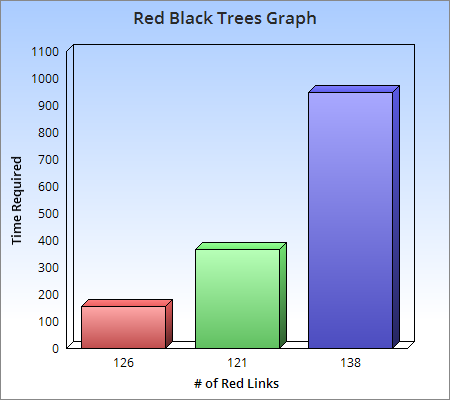
\includegraphics[width=15cm]{ChartGo.png}
\end{center}
\newpage
\begin{center}
\textbf{Part Three: While You Have Some Downtime}
\end{center}
\begin{enumerate}
\item In a Binary Search Tree, is the \textbf{delete()} operation commutative? (Does deleting x then y always give the same resulting tree as deleting y then x? Give an example to back up your answer.


\tikzstyle{line} = [draw, -latex']
\begin{tikzpicture}[->,>=stealth',level/.style={sibling distance = 1cm/#1,
  level distance = 1.5cm}] 
\node(first) [1] {$5$}
    child{ node [1] {$2$} 
            child{ node [1] {$1$} 
                         {}} %for a named pointer
            child{ node [1] {$4$}
            	child{ node[1]{$3$}        
         }
         }   
    };
\node(second) [1, right of=first, node distance=3cm] {$5$}
    child{ node [1] {$2$} 
                         {}} %for a named pointer
            child{ node [1] {$4$}
            	child{ node[1]{$3$} 
            	}
            	};
            	\node(third) [1, right of=second, node distance=3cm] {$5$}
            child{ node [1] {$4$}
            	child{ node[1]{$3$} 
            	}
            	};
\path [line] (first) -- node{Delete 1}(second);  
\path [line](second) -- node{Delete 2}(third);
\end{tikzpicture}
\\
\\
\begin{tikzpicture}[->,>=stealth',level/.style={sibling distance = 1cm/#1,
  level distance = 1.5cm}] 
\node(first) [1] {$5$}
    child{ node [1] {$2$} 
            child{ node [1] {$1$} 
                         {}} %for a named pointer
            child{ node [1] {$4$}
            	child{ node[1]{$3$}        
         }
         }   
    };
\node(second) [1, right of=first, node distance=3cm] {$5$}
    child{ node [1] {$3$}  
		child {node [1] {$1$}
		{}}
		child {node[1] {$4$}
    }};
    \node(third) [1, right of=second, node distance=3cm] {$5$}
    child{ node [1] {$3$}  
		child {node[1] {$4$}
    }};
                        
     

\path [line] (first) -- node{Delete 2}(second);  
\path [line] (second) -- node{Delete 1}(third);  
\end{tikzpicture}



\item Draw the 2-3 Tree that results when you insert the keys REDBLACKXYZ in that order into an initially empty tree.

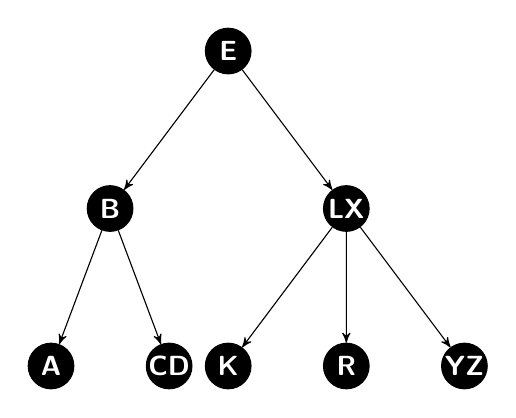
\begin{tikzpicture}[->,>=stealth',level/.style={sibling distance = 3cm/#1,
  level distance = 2cm}] 
\node [1] {E}
    child{ node [1] {B} 
    		child{ node[1] {A}}
    		child {node[1] {CD}}}
            child{ node [1] {LX}
            child{ node[1] {K}}
            child {node[1]{R}}
            child {node[1]{YZ}}}
            ;
                       
\end{tikzpicture}
\newpage
\item Draw the Red-Black that results from inserting the keys ABCDEFGHIJK in order into an initially empty tree. What happens in general when trees are build by inserting keys in ascending order?

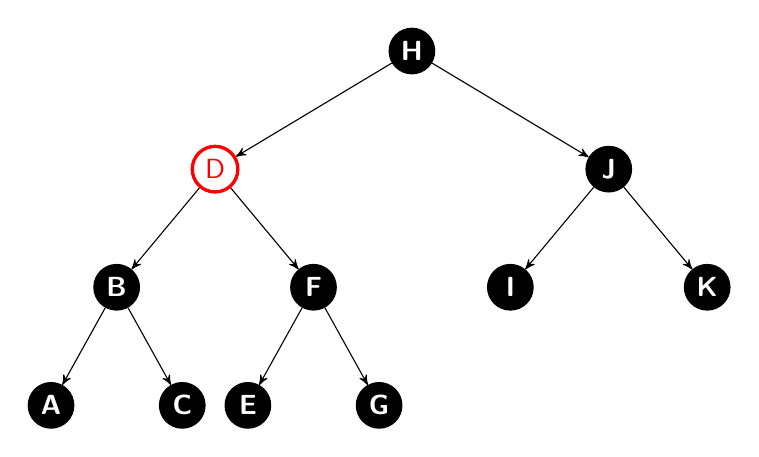
\begin{tikzpicture}[->,>=stealth',level/.style={sibling distance = 5cm/#1,
  level distance = 1.5cm}] 
\node [arn_n] {H}
    child{ node [arn_r] {D} 
            child{ node [arn_n] {B} 
            	child{ node [arn_n] {A} edge from parent node[above left]
                         {}} %for a named pointer
							child{ node [arn_n] {C}}
            }
            child{ node [arn_n] {F}
							child{ node [arn_n] {E}}
							child{ node [arn_n] {G}}
            }                            
    }
    child{ node [arn_n] {J}
            child{ node [arn_n] {I} 
            }
            child{ node [arn_n] {K}
            }
		}
; 
\end{tikzpicture}
\\
In general, when trees are build by inserting keys in ascending order, one has a lot of fun performing red black trees. Since it is in ascending order, at first we will try to insert the next character to the left since it is greater but this does not work since red links can never go right, they always have to go left. Since they have to go left, one would have to either perform the method rotateLeft(), rotateRight(), and flipColors().


\item Find a sequence of keys to insert into a Binary Search Tree and into a Red-Black Tree such that the height of the Binary Search Tree is less than the height of the Red-Black Tree. Alternatively, prove that no such sequence of keys is possible.
\\
\\
This is no sequence of keys to insert into both a Binary Search Tree and Red-Black Tree where the height of the Binary Search Tree is less than the height of the Red-Black Tree. This sequence is not possible due to the fact that Red-Black Trees are trees that have to be balanced. Since they have to balanced, then the same height on the right side will be equal to the same height on the left side. In a binary-search tree, these trees do not have to be balanced. A sequence of keys could be inserted where every keys is less than so that the height is going to be  greater than the Red Black Trees.




\end{enumerate}



\end{document}